\documentclass[12pt, titlepage]{article}
\usepackage{beamerarticle}
\usepackage[utf8]{inputenc}
\usepackage{hyperref}
\usepackage{amssymb,amsmath}

% Page settings
\usepackage[letterpaper, margin=1in]{geometry}
\usepackage{times}
%\usepackage{palatino}%\usepackage{lmodern, times}
%\usepackage{lmodern}%\usepackage{lmodern, times}
\usepackage{setspace}                           
\onehalfspacing %\doublespacing  % \singlespacing 

% Appendix
\usepackage{appendix}

% Line numbers
%\usepackage{lineno}
%\linenumbers


% Tables
\usepackage{array,booktabs,longtable,rotating}
\newenvironment{tablenotes}[1][]{
  \begin{minipage}{\textwidth}\emph{Notes:}{\footnotesize #1}
}{\end{minipage}}
\makeatletter
\def\fps@table{htbp}
\makeatother

% Graphics
\usepackage{graphicx,grffile}
\makeatletter
\def\maxwidth{\ifdim\Gin@nat@width>\linewidth\linewidth\else\Gin@nat@width\fi}
\def\maxheight{\ifdim\Gin@nat@height>\textheight\textheight\else\Gin@nat@height\fi}
\makeatother
% Scale images if necessary, so that they will not overflow the page
% margins by default, and it is still possible to overwrite the defaults
% using explicit options in \includegraphics[width, height, ...]{}
\setkeys{Gin}{width=\maxwidth,height=\maxheight,keepaspectratio}
% set default figure placement to htbp
\makeatletter
\def\fps@figure{htbp}
\makeatother

\usepackage{natbib}% plainnat
\bibliographystyle{abbrvnat}
\setcitestyle{authoryear,open={(},close={)}}
%\bibliographystyle{aer}
\usepackage{color}
\usepackage{fancyvrb}
\newcommand{\VerbBar}{|}
\newcommand{\VERB}{\Verb[commandchars=\\\{\}]}
\DefineVerbatimEnvironment{Highlighting}{Verbatim}{commandchars=\\\{\}}
% Add ',fontsize=\small' for more characters per line
\usepackage{framed}
\definecolor{shadecolor}{RGB}{255,255,255}
\newenvironment{Shaded}{\begin{snugshade}}{\end{snugshade}}
\newcommand{\KeywordTok}[1]{\textcolor[rgb]{0.12,0.11,0.11}{\textbf{#1}}}
\newcommand{\DataTypeTok}[1]{\textcolor[rgb]{0.00,0.34,0.68}{#1}}
\newcommand{\DecValTok}[1]{\textcolor[rgb]{0.69,0.50,0.00}{#1}}
\newcommand{\BaseNTok}[1]{\textcolor[rgb]{0.69,0.50,0.00}{#1}}
\newcommand{\FloatTok}[1]{\textcolor[rgb]{0.69,0.50,0.00}{#1}}
\newcommand{\ConstantTok}[1]{\textcolor[rgb]{0.67,0.33,0.00}{#1}}
\newcommand{\CharTok}[1]{\textcolor[rgb]{0.57,0.30,0.62}{#1}}
\newcommand{\SpecialCharTok}[1]{\textcolor[rgb]{0.24,0.68,0.91}{#1}}
\newcommand{\StringTok}[1]{\textcolor[rgb]{0.75,0.01,0.01}{#1}}
\newcommand{\VerbatimStringTok}[1]{\textcolor[rgb]{0.75,0.01,0.01}{#1}}
\newcommand{\SpecialStringTok}[1]{\textcolor[rgb]{1.00,0.33,0.00}{#1}}
\newcommand{\ImportTok}[1]{\textcolor[rgb]{1.00,0.33,0.00}{#1}}
\newcommand{\CommentTok}[1]{\textcolor[rgb]{0.54,0.53,0.53}{#1}}
\newcommand{\DocumentationTok}[1]{\textcolor[rgb]{0.38,0.47,0.50}{#1}}
\newcommand{\AnnotationTok}[1]{\textcolor[rgb]{0.79,0.38,0.79}{#1}}
\newcommand{\CommentVarTok}[1]{\textcolor[rgb]{0.00,0.58,1.00}{#1}}
\newcommand{\OtherTok}[1]{\textcolor[rgb]{0.00,0.43,0.16}{#1}}
\newcommand{\FunctionTok}[1]{\textcolor[rgb]{0.39,0.29,0.61}{#1}}
\newcommand{\VariableTok}[1]{\textcolor[rgb]{0.00,0.34,0.68}{#1}}
\newcommand{\ControlFlowTok}[1]{\textcolor[rgb]{0.12,0.11,0.11}{\textbf{#1}}}
\newcommand{\OperatorTok}[1]{\textcolor[rgb]{0.12,0.11,0.11}{#1}}
\newcommand{\BuiltInTok}[1]{\textcolor[rgb]{0.39,0.29,0.61}{\textbf{#1}}}
\newcommand{\ExtensionTok}[1]{\textcolor[rgb]{0.00,0.58,1.00}{\textbf{#1}}}
\newcommand{\PreprocessorTok}[1]{\textcolor[rgb]{0.00,0.43,0.16}{#1}}
\newcommand{\AttributeTok}[1]{\textcolor[rgb]{0.00,0.34,0.68}{#1}}
\newcommand{\RegionMarkerTok}[1]{\textcolor[rgb]{0.00,0.34,0.68}{#1}}
\newcommand{\InformationTok}[1]{\textcolor[rgb]{0.69,0.50,0.00}{#1}}
\newcommand{\WarningTok}[1]{\textcolor[rgb]{0.75,0.01,0.01}{#1}}
\newcommand{\AlertTok}[1]{\textcolor[rgb]{0.75,0.01,0.01}{\textbf{#1}}}
\newcommand{\ErrorTok}[1]{\textcolor[rgb]{0.75,0.01,0.01}{\underline{#1}}}
\newcommand{\NormalTok}[1]{\textcolor[rgb]{0.12,0.11,0.11}{#1}}


\setlength{\emergencystretch}{3em}  % prevent overfull lines
\providecommand{\tightlist}{%
  \setlength{\itemsep}{0pt}\setlength{\parskip}{0pt}}



\institute{}
\titlegraphic{}

\usepackage{xcolor}
\newcommand\todonote[1]{\textcolor{red}{#1}}



% Subscript
\newcommand\sub[1]{_{#1}}
\newcommand\supsc[1]{^{#1}}

\title{Survey HeroX}
\author{Preliminary data analysis}
\date{This version: \today}

\begin{document}
\maketitle


% Todo notes
%\usepackage[textsize=tiny]{todonotes}
%\newcommand\redmarginpar[1]{\marginpar{\footnotesize{\textcolor{red}{#1}}}}
%\listoftodos[Notes]
\clearpage

\begin{verbatim}
## [1] "Survey respondents=84"
\end{verbatim}

\begin{verbatim}
## [1] "56 percent of target (target=150)"
\end{verbatim}

\begin{verbatim}
## [1] "3 percent of respodents over solicited (solicited=3,154)"
\end{verbatim}

\begin{Shaded}
\begin{Highlighting}[]
\KeywordTok{attach}\NormalTok{(survey)}

\CommentTok{# Age}
\KeywordTok{pie}\NormalTok{(}\KeywordTok{table}\NormalTok{(QID3), }\DataTypeTok{main=}\NormalTok{questions[}\StringTok{"QID3"}\NormalTok{])}
\end{Highlighting}
\end{Shaded}

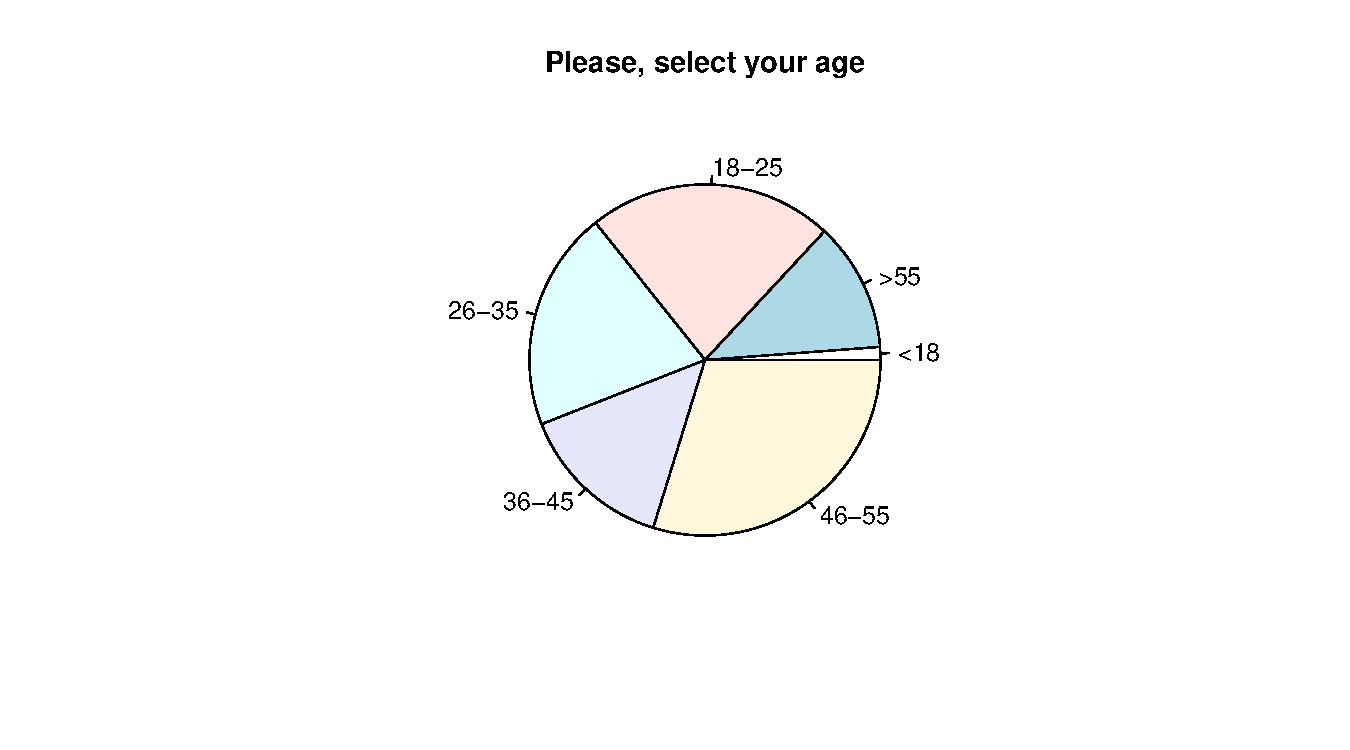
\includegraphics{analysis_survey_files/figure-latex/unnamed-chunk-2-1.pdf}

\begin{Shaded}
\begin{Highlighting}[]
\CommentTok{# Gender}
\KeywordTok{pie}\NormalTok{(}\KeywordTok{table}\NormalTok{(QID4), }\DataTypeTok{main=}\NormalTok{questions[}\StringTok{"QID4"}\NormalTok{])}
\end{Highlighting}
\end{Shaded}

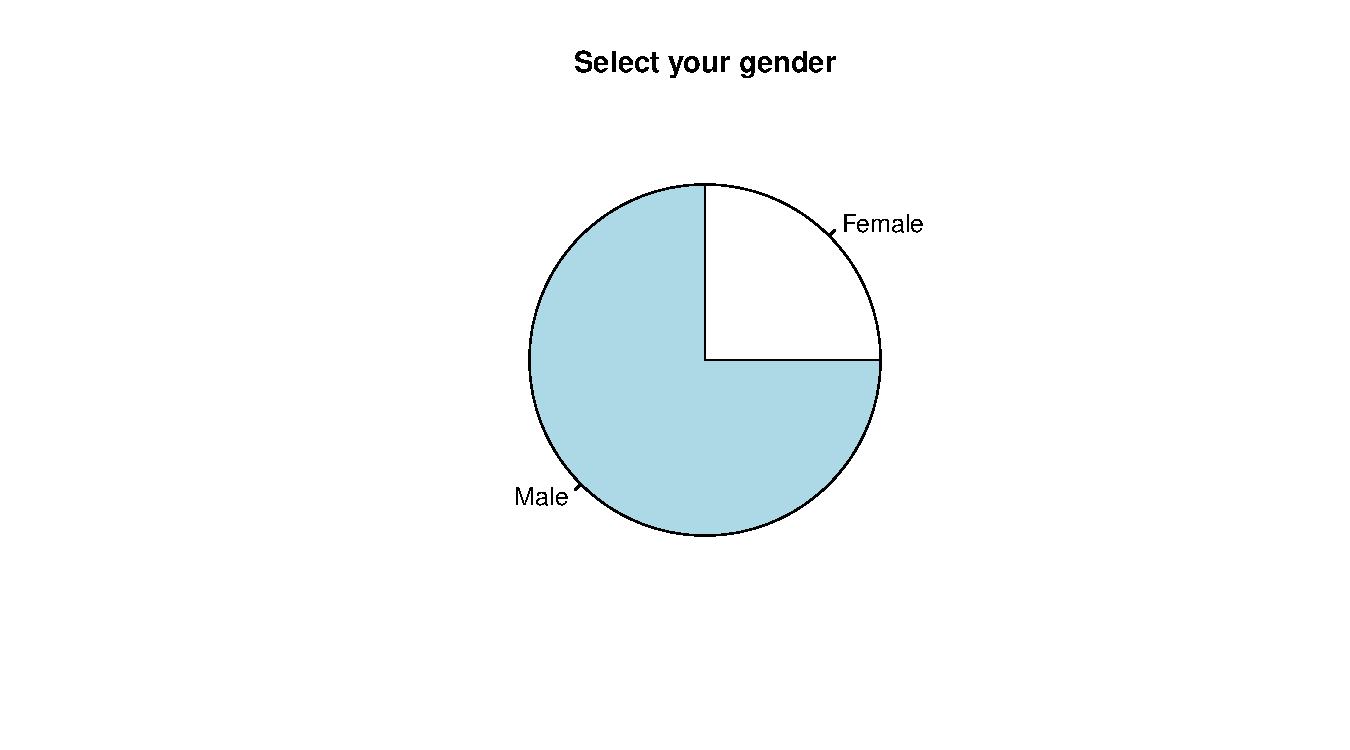
\includegraphics{analysis_survey_files/figure-latex/unnamed-chunk-2-2.pdf}

\begin{Shaded}
\begin{Highlighting}[]
\CommentTok{# Country}
\KeywordTok{pie}\NormalTok{(}\KeywordTok{table}\NormalTok{(QID5), }\DataTypeTok{main=}\NormalTok{questions[}\StringTok{"QID5"}\NormalTok{])}
\end{Highlighting}
\end{Shaded}

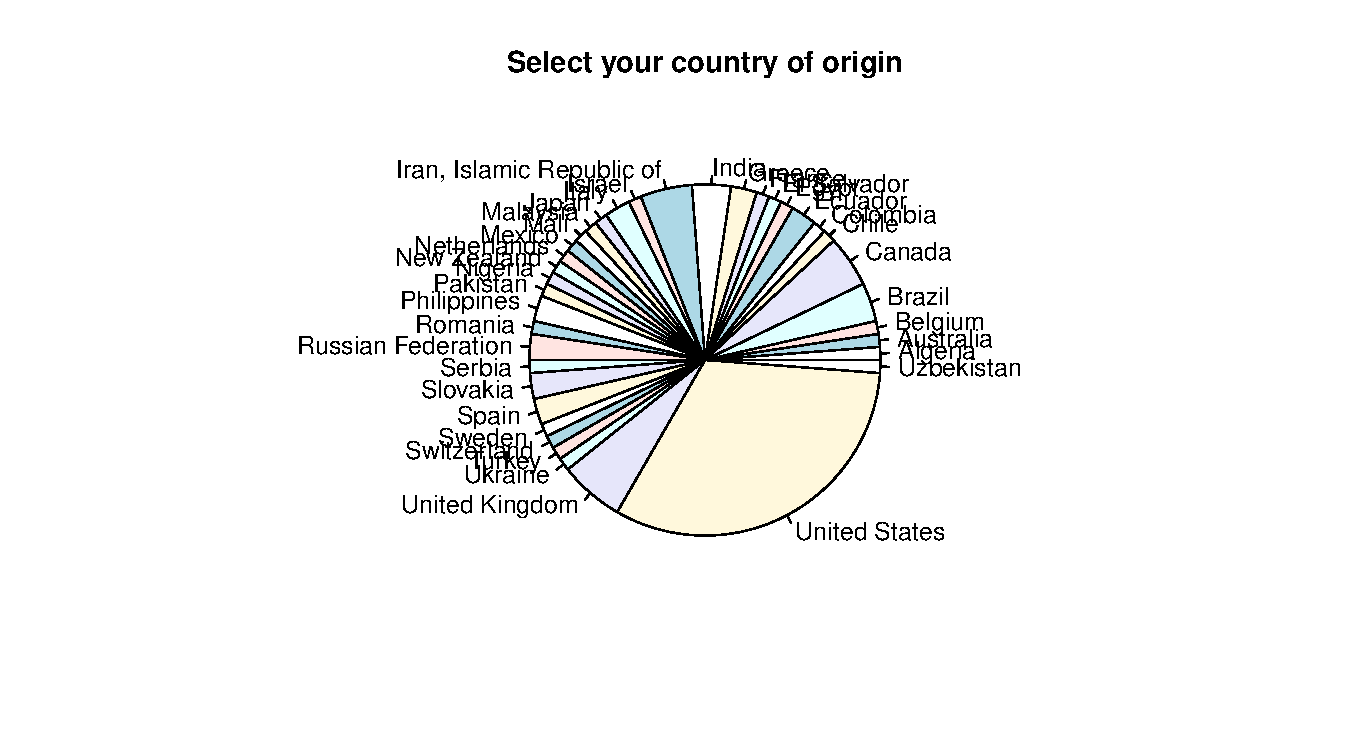
\includegraphics{analysis_survey_files/figure-latex/unnamed-chunk-2-3.pdf}

\begin{Shaded}
\begin{Highlighting}[]
\CommentTok{# Education}
\KeywordTok{pie}\NormalTok{(}\KeywordTok{table}\NormalTok{(Q22), }\DataTypeTok{main=}\NormalTok{questions[}\StringTok{"Q22"}\NormalTok{])}
\end{Highlighting}
\end{Shaded}

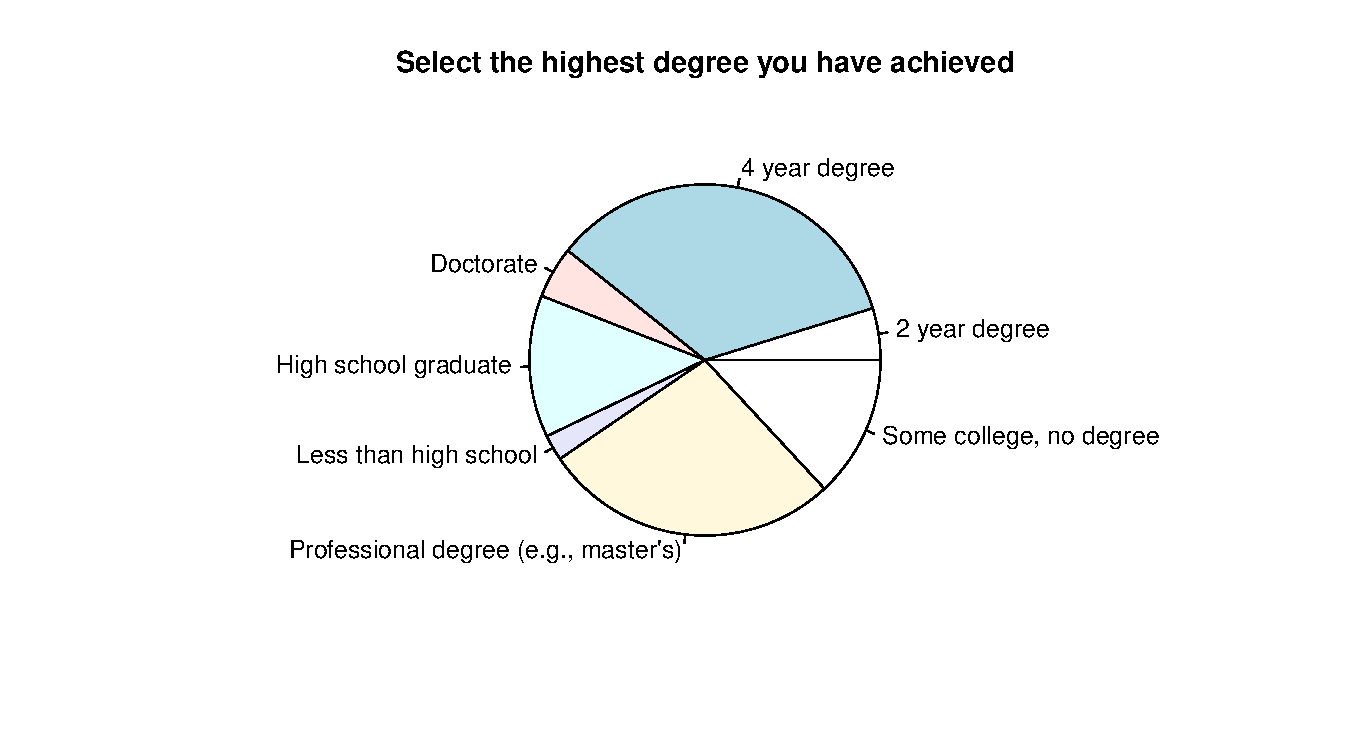
\includegraphics{analysis_survey_files/figure-latex/unnamed-chunk-2-4.pdf}

\begin{Shaded}
\begin{Highlighting}[]
\CommentTok{# Employment}
\KeywordTok{pie}\NormalTok{(}\KeywordTok{table}\NormalTok{(Q23), }\DataTypeTok{main=}\NormalTok{questions[}\StringTok{"Q23"}\NormalTok{])}
\end{Highlighting}
\end{Shaded}

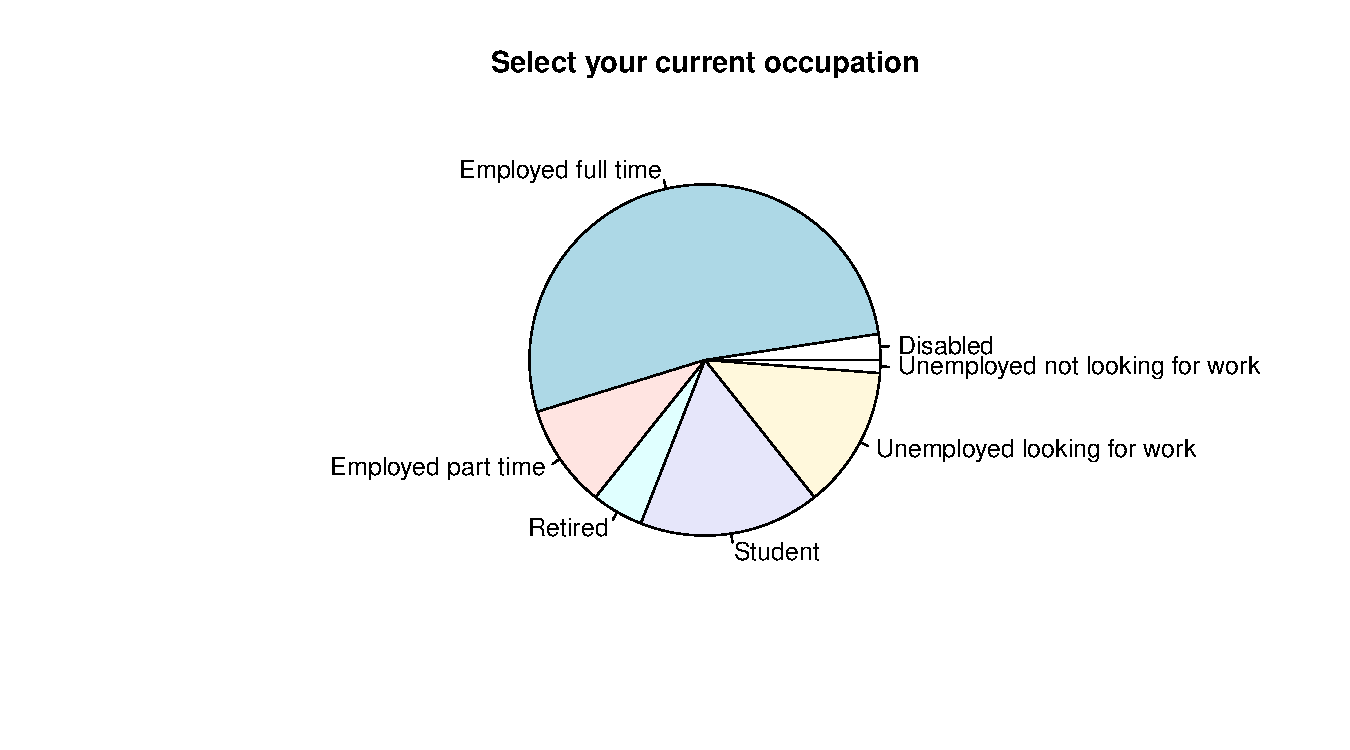
\includegraphics{analysis_survey_files/figure-latex/unnamed-chunk-2-5.pdf}

\begin{Shaded}
\begin{Highlighting}[]
\CommentTok{# Motivations}
\KeywordTok{pie}\NormalTok{(}\KeywordTok{table}\NormalTok{(QID6), }\DataTypeTok{main=}\NormalTok{questions[}\StringTok{"QID6"}\NormalTok{])}
\end{Highlighting}
\end{Shaded}

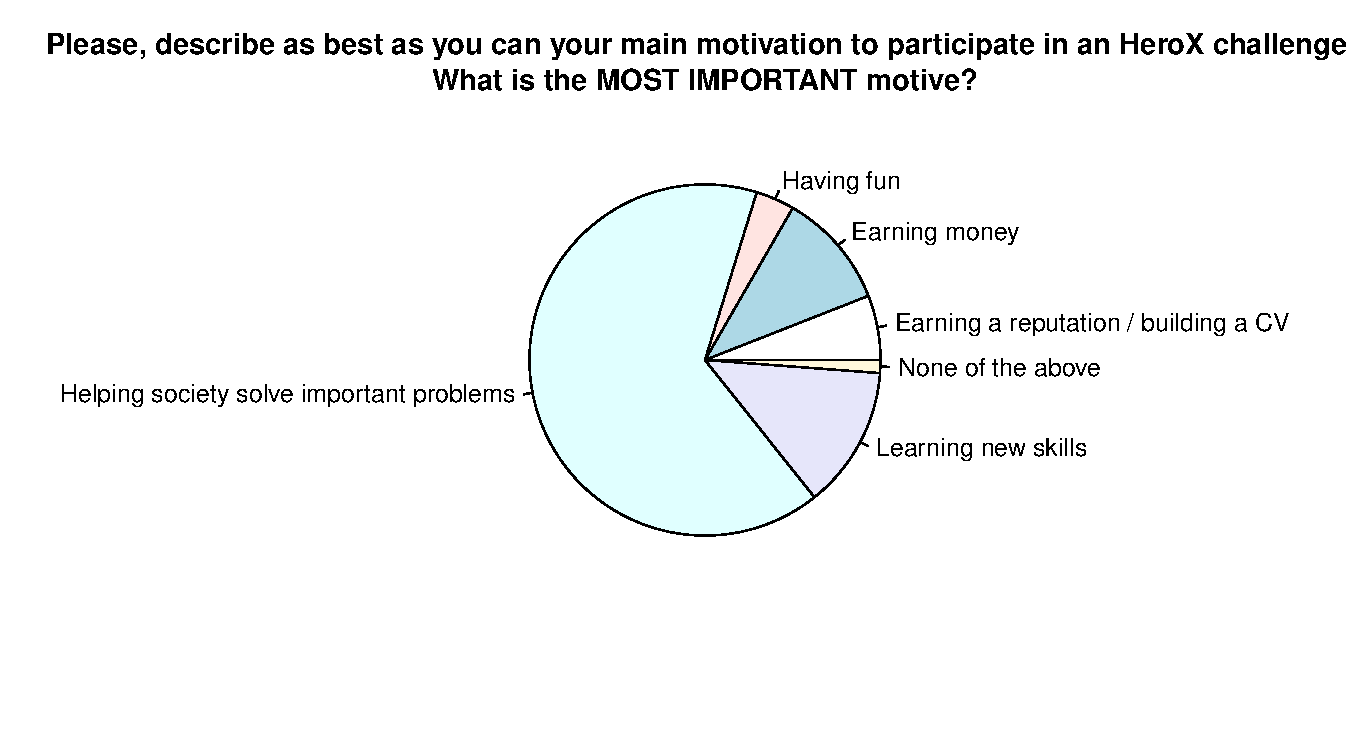
\includegraphics{analysis_survey_files/figure-latex/unnamed-chunk-2-6.pdf}

\begin{Shaded}
\begin{Highlighting}[]
\CommentTok{# Competitive}
\KeywordTok{pie}\NormalTok{(}\KeywordTok{table}\NormalTok{(QID7), }\DataTypeTok{main=}\NormalTok{questions[}\StringTok{"QID7"}\NormalTok{])}
\end{Highlighting}
\end{Shaded}

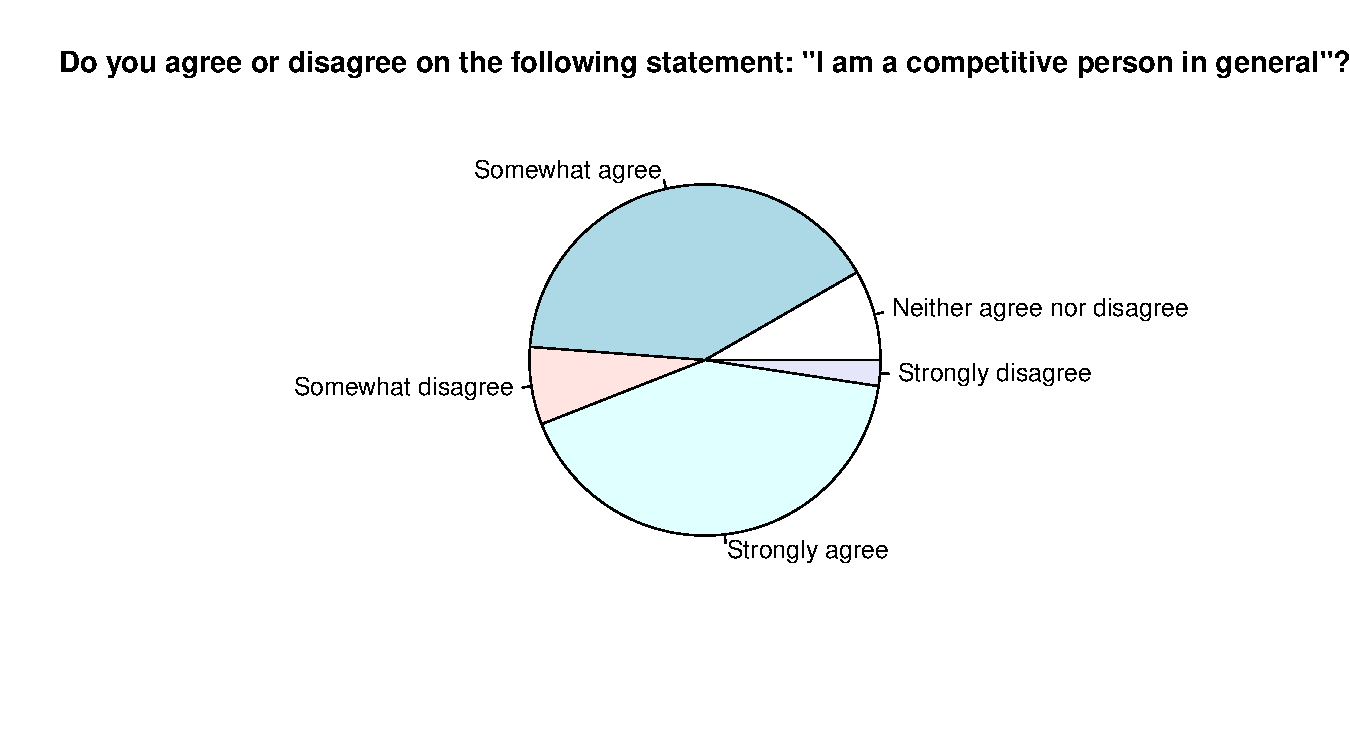
\includegraphics{analysis_survey_files/figure-latex/unnamed-chunk-2-7.pdf}

\begin{Shaded}
\begin{Highlighting}[]
\CommentTok{# Teams}
\KeywordTok{pie}\NormalTok{(}\KeywordTok{table}\NormalTok{(QID8), }\DataTypeTok{main=}\NormalTok{questions[}\StringTok{"QID8"}\NormalTok{])}
\end{Highlighting}
\end{Shaded}

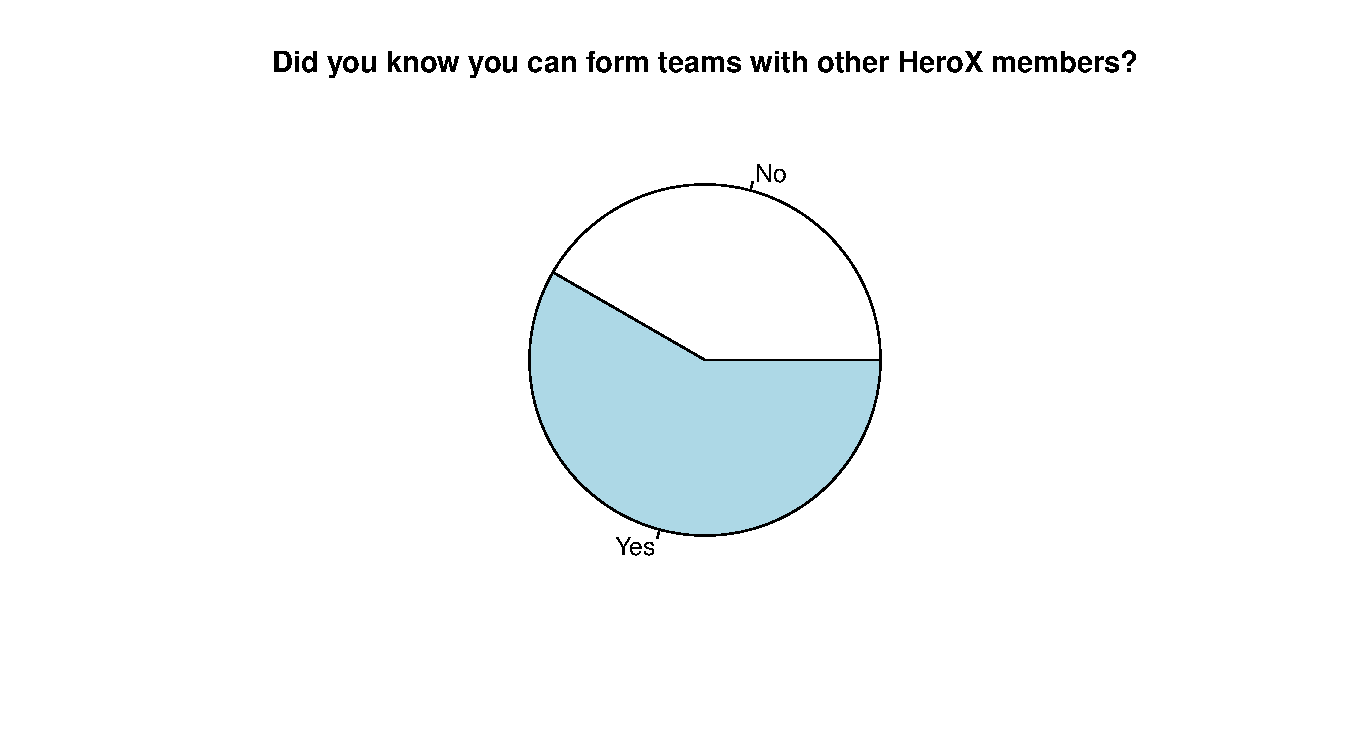
\includegraphics{analysis_survey_files/figure-latex/unnamed-chunk-2-8.pdf}

\begin{Shaded}
\begin{Highlighting}[]
\KeywordTok{pie}\NormalTok{(}\KeywordTok{table}\NormalTok{(QID9), }\DataTypeTok{main=}\KeywordTok{strnl}\NormalTok{(questions[}\StringTok{"QID9"}\NormalTok{]))}
\end{Highlighting}
\end{Shaded}

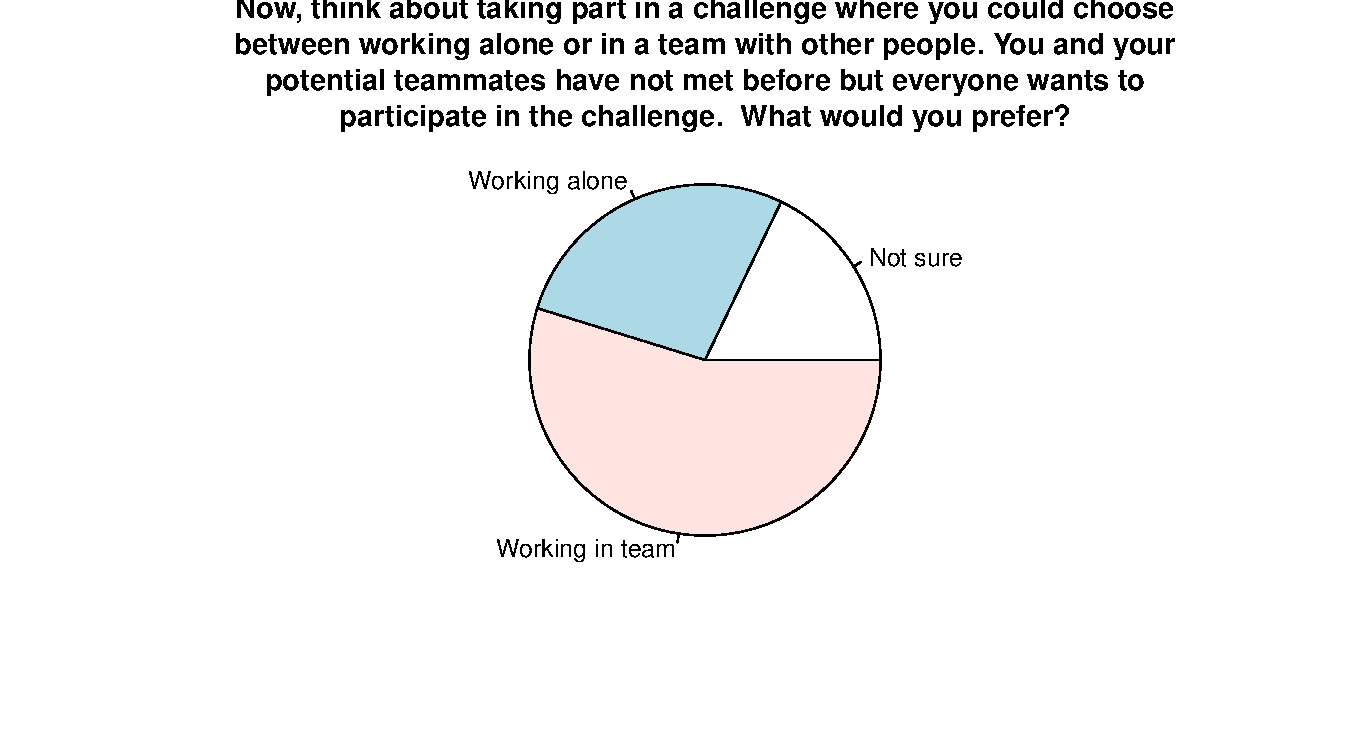
\includegraphics{analysis_survey_files/figure-latex/unnamed-chunk-2-9.pdf}

\begin{Shaded}
\begin{Highlighting}[]
\CommentTok{# Teams composition}
\KeywordTok{pie}\NormalTok{(}\KeywordTok{table}\NormalTok{(Q13), }\DataTypeTok{main=}\KeywordTok{strnl}\NormalTok{(questions[}\StringTok{"Q13"}\NormalTok{]))}
\end{Highlighting}
\end{Shaded}

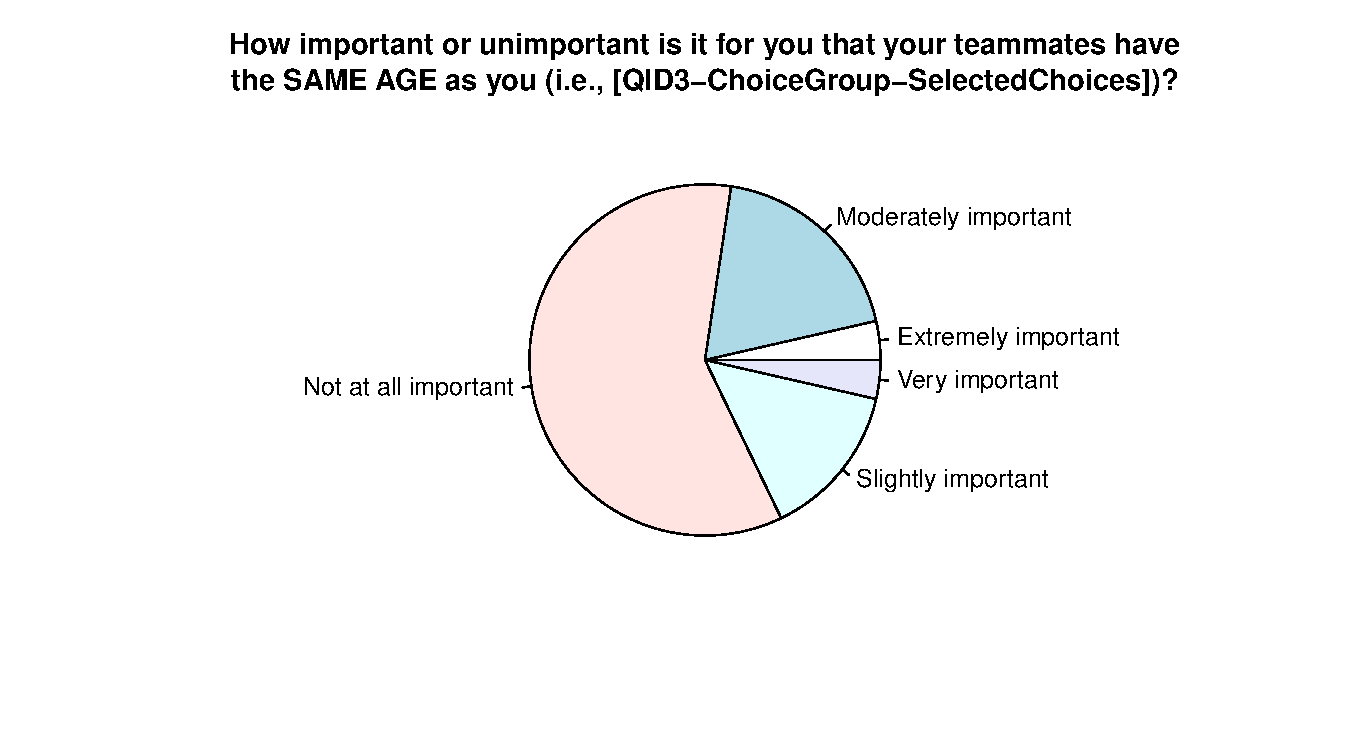
\includegraphics{analysis_survey_files/figure-latex/unnamed-chunk-2-10.pdf}

\begin{Shaded}
\begin{Highlighting}[]
\KeywordTok{pie}\NormalTok{(}\KeywordTok{table}\NormalTok{(Q15), }\DataTypeTok{main=}\KeywordTok{strnl}\NormalTok{(questions[}\StringTok{"Q15"}\NormalTok{]))}
\end{Highlighting}
\end{Shaded}

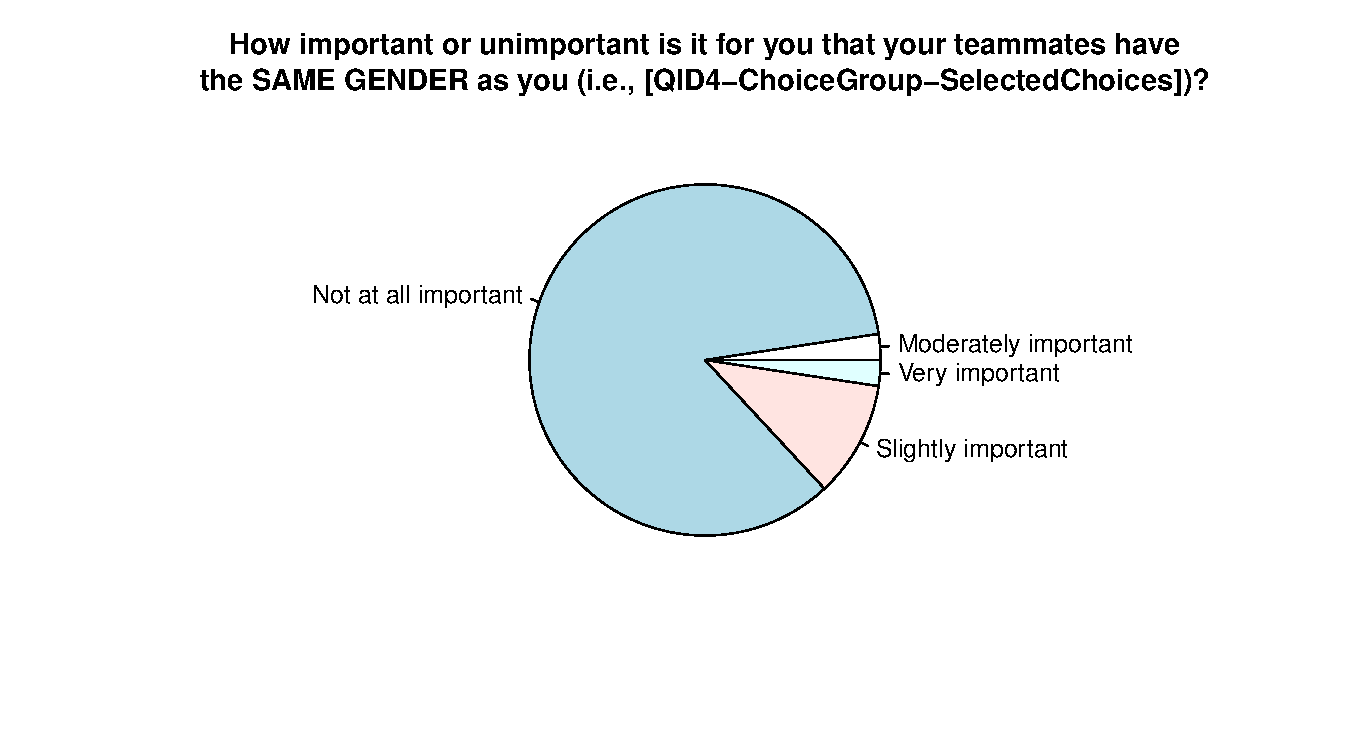
\includegraphics{analysis_survey_files/figure-latex/unnamed-chunk-2-11.pdf}

\begin{Shaded}
\begin{Highlighting}[]
\KeywordTok{pie}\NormalTok{(}\KeywordTok{table}\NormalTok{(Q16), }\DataTypeTok{main=}\KeywordTok{strnl}\NormalTok{(questions[}\StringTok{"Q16"}\NormalTok{]))}
\end{Highlighting}
\end{Shaded}

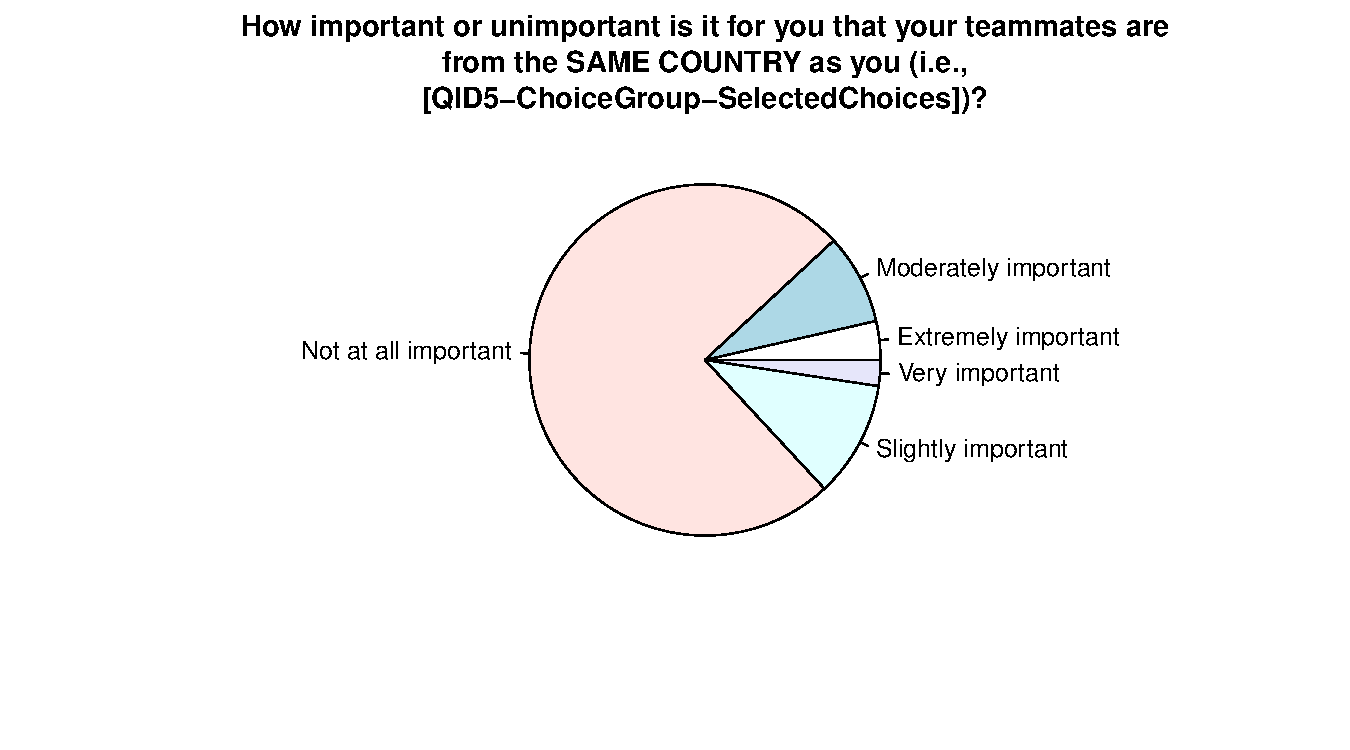
\includegraphics{analysis_survey_files/figure-latex/unnamed-chunk-2-12.pdf}

\begin{Shaded}
\begin{Highlighting}[]
\CommentTok{# pie(table(Q17), main=questions["Q17"])}
\KeywordTok{plot}\NormalTok{(}\KeywordTok{table}\NormalTok{(Q18, QID4), }\DataTypeTok{main=}\KeywordTok{strnl}\NormalTok{(questions[}\StringTok{"Q18"}\NormalTok{]), }\DataTypeTok{col=}\KeywordTok{c}\NormalTok{(}\StringTok{"dodgerblue"}\NormalTok{, }\StringTok{"orange"}\NormalTok{))}
\end{Highlighting}
\end{Shaded}

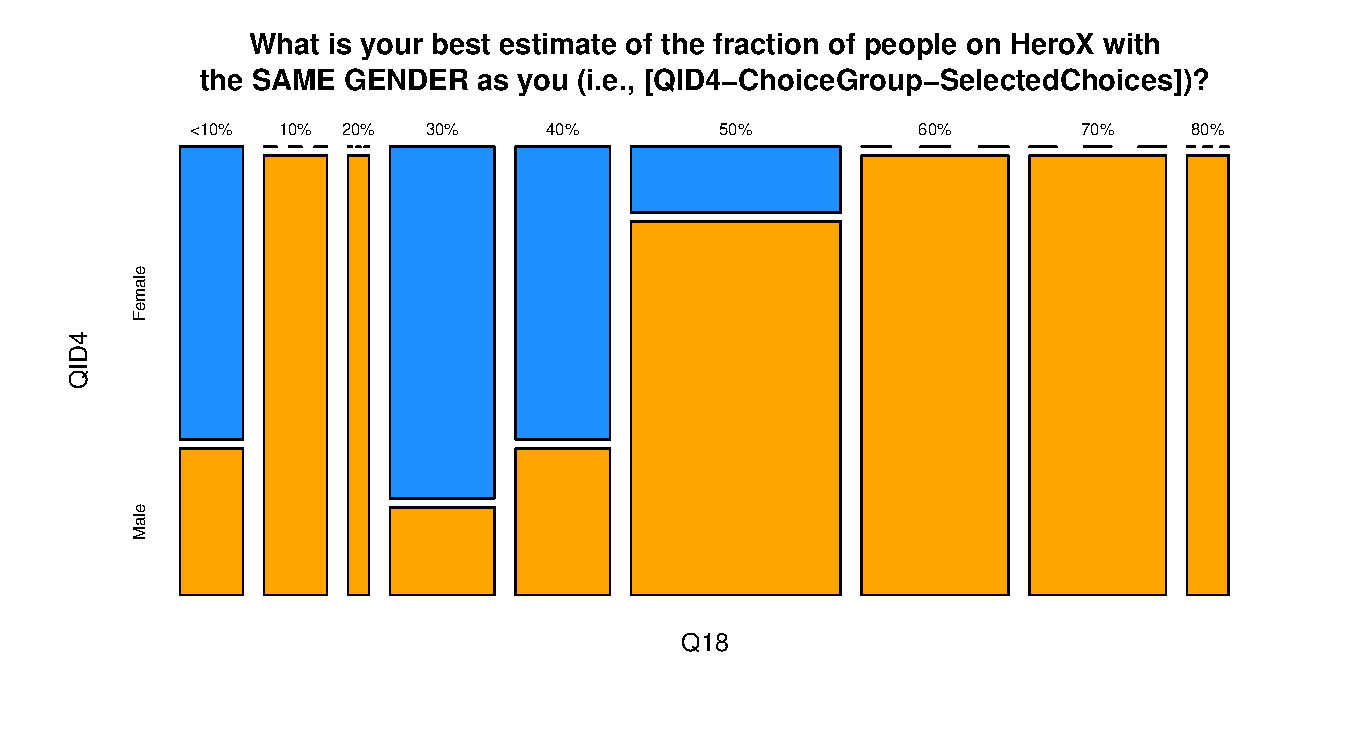
\includegraphics{analysis_survey_files/figure-latex/unnamed-chunk-2-13.pdf}

\begin{Shaded}
\begin{Highlighting}[]
\CommentTok{# Areas}
\KeywordTok{pie}\NormalTok{(}\KeywordTok{sort}\NormalTok{(}\KeywordTok{table}\NormalTok{(}\KeywordTok{unlist}\NormalTok{(}\KeywordTok{strsplit}\NormalTok{(}\KeywordTok{as.character}\NormalTok{(QID12), }\StringTok{","}\NormalTok{)))))}
\end{Highlighting}
\end{Shaded}

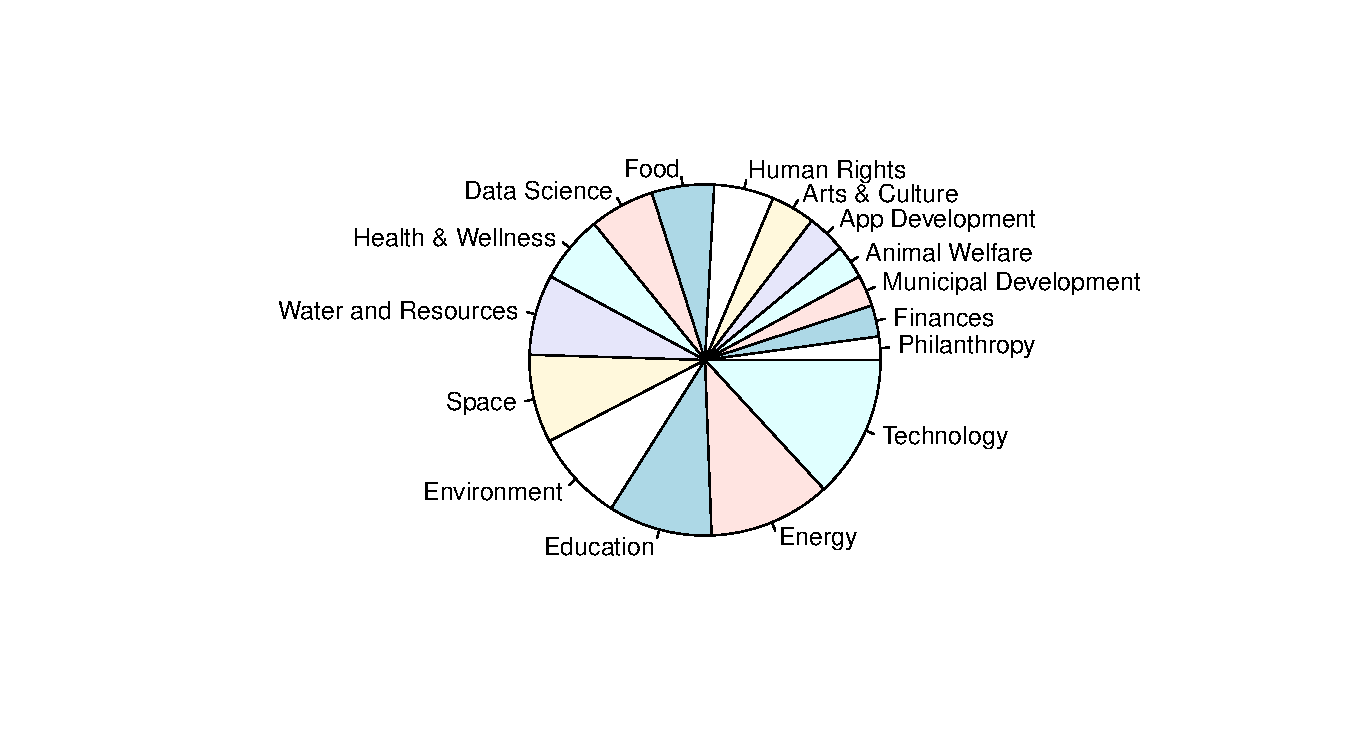
\includegraphics{analysis_survey_files/figure-latex/unnamed-chunk-2-14.pdf}

\bibliography{library.bib}

\end{document}